
\section{Entdeckung des Top-Quarks}

\chapterauthor{Alexnder Froch, 18.01.2019}

\subsection{Übersicht der Entdeckung}

Das Top-Quark ist eines der beiden Quarks der dritten Generation und mit einer heute bekannten Masse von  $m_t = \SI{173.1(6)}{\giga\electronvolt}$ das schwerste bekannte Quark und Elementarteilchen.
Bereits im Jahre 1973 postulierten Kobayashi und Maswaka sowohl das Bottom-Quark als auch das Top-Quark theoretisch um die beobachtete CP-Verletzung beim Zerfall von Kaonen zu erklären.
Sie erhielten nach der Entdeckung des b-Quarks 1977 am Fermilab sowie des t-Quarks 1995 am Tevatron im Jahre 2008 den Nobelpreis.

Die tatsächliche Entdeckung des b-Quarks 1977 gab Anlass zur Suche nach dem t-Quark.
Im Jahre 1984 konnte durch die erfolglose direkte Suche am SLAC ein unteres Limit von \SI{23.3}{\giga\electronvolt} auf die Topmasse gegeben werden.
Die Ergebnisse des ARGUS Experiment am DESY, welches Oszillationen von B-Mesonen untersuchte, wiesen 1987 aufgrund der gemessenen Oszillationsfrequenzen, welche sensitiv auf die Topquarkmasse sind, auf eine Masse von über \SI{50}{\giga\electronvolt} hin.
Die Ergebnisse von VENUS am KEK, OPAL am LEP sowie UA2 am Sp$\overline{\text{p}}$S konnten durch weitere Suche in direkter Produktion diese Ergebnisse von ARGUS bestätigen und ebenfalls untere Limits setzen. 
Die schlussendliche Entdeckung gelang im Jahre 1995 dem Tevatron mit den Experimenten CDF und D0.

\subsection{Theorie und indirekte Messungen}

Als Produktionskanäle für das Topquark kommen insbesondere Gluon-Gluon Fusion, zwei Gluonen in einem t-Kanal sowie die Annihilation von $q\overline{q}$ infrage, wobei jeweils ein t$\overline{t}$-Paar entsteht.
Auch die Produktion von einzelnen t-Quarks ist möglich, beispielsweise über $q\overline{q}$-Annihilation oder weitere Prozesse der schwachen Wechselwirkung mit $b$-Quarks.
Die Lebenszeit von Top-Quarks ist zu gering um Baryonen zu bilden, so dass das Top primär in ein Bottom-Quark sowie ein W-Boson zerfällt.

Aus theoretischer Sicht ist das Top-Quark ebenfalls interessant zu untersuchen:
Aufgrund seiner hohen Masse koppelt es besonders stark an das Higgs-Boson und ist somit hochsensitiv auf ggf. vorhandene neue Physik, siehe auch Kapitel \ref{sec:higgs}.

Erste Hinweise auf das Vorhandensein eines Top-Quarks kann der sogenannte R-Plot geben, welcher das Verhältnis
\begin{align*}
	R = \frac{\sigma\left( e^+ e^- \rightarrow \text{Hadronen} \right)}{\sigma \left( e^+ e^- \rightarrow \mu^+ \mu^- \right)}
\end{align*}
in Abhängigkeit von der Schwerpunktsenergie angibt.
So verändert sich der Faktor $R$ mit der Schwerpunktsenergie wenn neue Quarks erzeugt weden können.
Zudem sind viele elektroschwache Variablen sensitiv auf die Topmasse so dass auch mit Messungen von diesen Variablen die Masse des Top-Quarks genauer bestimmt werden konnte.

\subsection{Entdeckung des Top-Quarks am Tevatron}

Der CDF-Detektor ist in Abbildung \ref{fig:cdf} dargestellt.
Der Detektoraufbau ist dabei insbesondere darauf ausgelegt mithilfe der Spurkammern sekundäre Vertices rekonstruieren  sowie mit den Kalorimetern Jet- und Hadronenenergien bestimmen zu können.
\begin{figure}
  \centering
  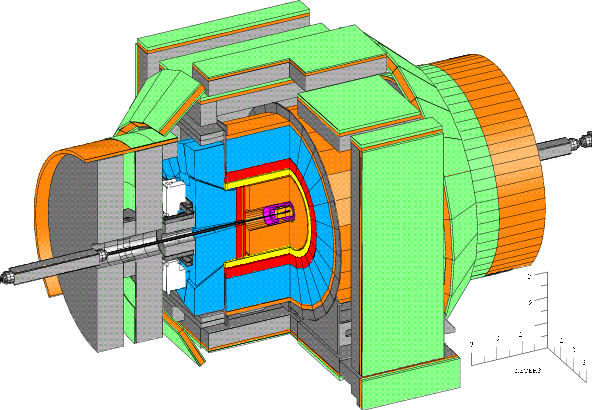
\includegraphics[height=6.0cm]{ressources/cdfii_3d_p1.png}
  \caption{CDF-Detektor, mit Spurkammern (orange), elektromagnetischen Kalorimeter (rot), hadronischem Kalorimeter (blau) und Myonkammern (grün) \cite{Galtieri:2011yd}}
  \label{fig:cdf}
\end{figure}
Die Analyse wurde anhand des Kanals $t \overline{t} \rightarrow W b W \overline{W}$ durchgeführt wobei Daten bei einer Schwerpunktsenergie von $\sqrt{s} = \SI{1.8}{\tera\electronvolt}$ aufgenommen wurden.
Bei den W-Bosonen wird dabei insbesondere der Zerfall in zwei Leptonen oder ein semileptonischer Zerfall betrachtet wobei dileptonische Ereignisse in bestimmen Energiebereichen verworfen wurden um direkt erzeuge W- und Z-Bosonen ausschließen zu können.
Um die $b$-Quarks rekonstruieren zu können wird ein SVX-Tagging durchgeführt wobei ein sekundärer Vertex durch den Zerfall des b-Quarks erwartet wird.
Um Untergründe zu unterdrücken wird eine Kombination der Rekonstruktion des Zerfallsvertices mit der Identifikation der enstehenden Leptonen genutzt.
Dabei sind bei letzterer Identifikation insbesondere Untergründe von Hadronen und Elektronen aus anderen, unbekannten Quellen zu berücksichtigen.
Die Wahrscheinlichkeit, dass es sich bei den Ergebnissen nicht um statistische Fluktuationen des Untergrundes handelt konnte vom CDF zu $\num{4.8}\sigma$ bestimmt werden.
Mithilfe eines negativen Log-Likelihoodfits konnte aus den rekonstruierten Massen die Topquarkmasse zu 
\begin{align*}
	m_{t, \text{CDF}} = \left( \num{176} \pm \num{8} \pm \num{10} \right) \si{\giga\electronvolt}
\end{align*}
bestimmt werden.

Der zweite Detektor am Tevatron, das D0-Experiment, besaß neben Driftkammern zur Spurrekonstruktion einen Übergangsstrahlungsdetektor zur Identifikation von Elektronen sowie eine vorwärtsgerichtete Driftkammer um Jets zu detektieren welche ein hohes $\eta$ besitzen.
Anhand von kinematischen Anforderungen an die Leptonen und Jets in den verschiedenen Kanälen konnten passende Events ausgewählt werden und zwischen Signal und Untergrund, welcher insbesondere durch Z-Produktion sowie andere starke Prozesse entsteht, unterschieden werden.
Schlussendlich konnte die Topmasse durch Untersuchung des Kanals $t\overline{t} \rightarrow W^+ W^- b \overline{b} \rightarrow l \nu q \overline{q} b \overline{b}$ zu
\begin{align*}
	m_{t, \text{D0}} = \left( 199 \pm 20 \pm 22 \right)\si{\giga\electronvolt}
\end{align*}
rekontruiert werden.
Diese Werte stimmen mit den Ergebnisen von CDF gut überein.

\subsection{Heutige Messungen und Ausblick der Topphysik}
\label{sec:higgs}

Mithilfe von heutigen Messungen, insbesondere am LHC, konnte der Wirkungsquerschnitt der $t\overline{t}$ Produktion sowie der Einzel-Top Wirkungsquerschnitt genauer bestimmt werden, so dass die Messungen mit der theoretischen Vorhersage übereinstimmen.
Vorherige, größere Unsicherheiten auf den Wirkungsquerschnitt waren insbesondere auf die großen Unsicherheiten auf die Luminosität am Tevatron zurückzuführen.
Auch die Masse des Topquarks wurde am LHC vom ATLAS-Experiment untersucht wobei aufgrund der guten Auflösung des vorhandenen elektromagnetischen Kalorimeters der Endzustand von Leptonen und Jets betrachtet wurde.

In aktuellen und zukünftigen Messungen wird insbesondere die Ankopplung an den Higgs-Sektor in der $t \overline{t} \text{H}$-Produktion untersucht.
Hierbei zeigen die gemessenen Wirkungsquerschnitte in den verschiedenen Kanälen, insbesondere aufgrund der fehlenden Statistik, nach wie vor große Fehler auf.
Neben den experimentellen Unsicherheiten treten jedoch auch größere theoretische Fehler, beispielsweise durch mögliche Korerkturen höherer Ordnung sowie Unsicherheiten in der Kopplungskonstante oder den Partonverteilungsfunktionen auf.
Aufgrund dieser Unsicherheiten können zum jetzigen Zeitpunkt keine Einflüsse durch neue Physik ausgeschlossen werden, möglich ist aber auch dass der Prozess theoretisch noch nicht vollständig verstanden wurde oder Monte-Carlo Simulationen noch korrigiert werden müssen.